%! Author = Juniell
%! Date = 11.05.2021

% Preamble
\documentclass[a4paper, 14pt]{extarticle}

% Packages
\usepackage[T2A]{fontenc}
\usepackage{natbib}
\usepackage{graphicx}
\usepackage[english, russian]{babel}
\usepackage{fontspec}
\usepackage{amsmath}
\usepackage{amsfonts}
\usepackage{amssymb}
\usepackage{amsthm}
\usepackage{mathtools}
\usepackage{mathrsfs}
\usepackage{fullpage}
\usepackage{ulem}
\usepackage{setspace}
\usepackage{listings}
\usepackage{indentfirst}
\usepackage[left=2cm,right=1.5cm,top=2cm,bottom=2cm]{geometry}
\usepackage{xcolor}
\usepackage{float}
\usepackage{csquotes}
\usepackage{hyperref}
\usepackage{graphics}

\definecolor{urlcolor}{HTML}{0000FF} % цвет ссылок
\definecolor{linkcolor}{HTML}{000000} % цвет гиперссылок
\hypersetup{pdfstartview=FitH, linkcolor=linkcolor, urlcolor=urlcolor, colorlinks=true}

\setmainfont{Times New Roman}
\setlength{\parindent}{5ex}
\setlength{\parskip}{1em}
\renewcommand{\baselinestretch}{1}

\graphicspath{{resources/Images}}

\definecolor{buzzlightyear}{HTML}{8757A5}
\definecolor{grass}{HTML}{738D06}
\definecolor{literal}{HTML}{F18A2B}
\definecolor{commentcolor}{HTML}{8E908B}

\lstdefinestyle{habrstyle}{
    backgroundcolor=\color{white},
    commentstyle=\color{commentcolor},
    keywordstyle=\bfseries\color{buzzlightyear},
    numberstyle=\tiny\color{commentcolor},
    stringstyle=\color{grass},
    basicstyle=\ttfamily\footnotesize,
    breakatwhitespace=false,
    breaklines=true,
    captionpos=b,
    keepspaces=true,
    numbers=left,
    numbersep=5pt,
    showspaces=false,
    showstringspaces=false,
    showtabs=false,
    tabsize=4,
    language=Python
}

\lstset{style=habrstyle}


% Document
\begin{document}
% Титульный лист
    \begin{center}
        \begin{center}
            \hfill \break
            \normalsize{Санкт-Петербургский государственный политехнический}\\
            \normalsize{университет Петра Великого}\\
            \hfill \break
            \normalsize{\textbf{Высшая школа интеллектуальных систем и}}\\
            \normalsize{\textbf{суперкомпьютерных технологий}}\\
            \hfill \break
            \hfill \break
            \hfill \break
            \hfill \break
            \hfill \break
            \normalsize{Отчёт по лабораторной работе №9}\\
            \normalsize{Дисциплина: Телекоммуникационные технологии}\\
            \normalsize{Тема: Дифференцирование и интегрирование}\\
        \end{center}
        \hfill \break
        \hfill \break
        \hfill \break
        \hfill \break
        \hfill \break
        \hfill \break
        \hfill \break
        \hfill \break
        \hfill \break
        \hfill \break
        \begin{tabbing}
            Выполнил студент гр. 3530901/80201 \`В.А. Пучкина\\
            \\
            Преподаватель: \`Н.В. Богач\\
        \end{tabbing}
        \hfill \break
        \hfill \break
        \hfill \break
        \hfill \break
        \begin{center}
            Санкт-Петербург\\
            2021
        \end{center}
        \thispagestyle{empty}
    \end{center}

% Оглавление
    \newpage
    \tableofcontents

% Список иллюстраций
    \newpage
    \listoffigures

% Список листингов
    \newpage
    \lstlistoflistings

% ---------------------------------------------- Упражнение 9.1 ----------------------------------------------
    \newpage
    \section{Упражнение 9.1}
    \label{sec:task1}

    В этом упражнении необходимо изучить примеры в файле \texttt{chap09.ipynb}.
    После этого заменим периодический пилообразный сигнал на непериодические данные Facebook, чтобы проверить,
    какие именно примеры перестанут работать корректно.

    Итак, все примеры были изучены. Перейдём к эксперименту. Считаем файл с данными Facebook и получим \texttt{wave}.

    \begin{lstlisting}[caption= Чтение файла и получение \texttt{wave}., label={lst:task1_in_wave}]
df = pandas.read_csv('resources/task1_FB_2.csv', header=0, parse_dates=[0])
ys = df['Close']
in_wave = Wave(ys, framerate=1)
in_wave.plot()
decorate(xlabel='Time (days)', ylabel='Price')  \end{lstlisting}

    \begin{figure}[h]
        \centering
        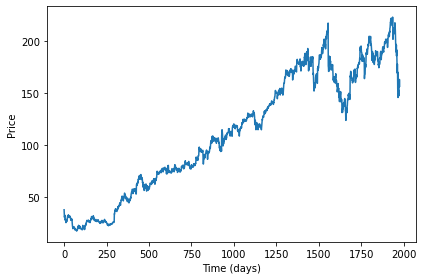
\includegraphics[width=0.8\linewidth]{resources/Images/task1_in_wave}
        \caption{Сигнал Facebook.}
        \label{fig:task1_in_wave}
    \end{figure}

    Теперь получим спектр нашего сигнала.

    \begin{lstlisting}[caption= Получение спектра сигнала Facebook., label={lst:task1_in_spectrum}]
in_spectrum = in_wave.make_spectrum()
in_spectrum.plot()
decorate(xlabel='Frequency (Hz)', ylabel='Amplitude')   \end{lstlisting}

    \begin{figure}[H]
        \centering
        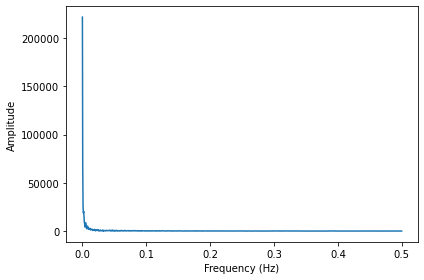
\includegraphics[width=0.7\linewidth]{resources/Images/task1_in_spectrum}
        \caption{Спектр сигнала Facebook.}
        \label{fig:task1_in_spectrum}
    \end{figure}

    Теперь рассчитаем выходной сигнал как совокупную сумму входных сигналов.

    \begin{lstlisting}[caption= Рассчёт выходного сигнала., label={lst:task1_out_wave}]
out_wave = in_wave.cumsum()
out_wave.unbias()
out_wave.plot()
decorate(xlabel='Time (s)') \end{lstlisting}

    \begin{figure}[H]
        \centering
        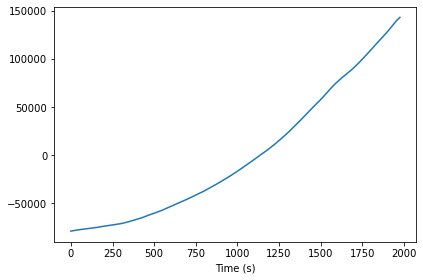
\includegraphics[width=0.7\linewidth]{resources/Images/task1_out_wave}
        \caption{Выходной сигнал.}
        \label{fig:task1_out_wave}
    \end{figure}

    И получим спектр выходного \texttt{wave}.

    \begin{lstlisting}[caption= Получение спектра выходного сигнала., label={lst:task1_out_spectrum}]
out_spectrum = out_wave.make_spectrum()
out_spectrum.plot()
decorate(xlabel='Frequency (Hz)', ylabel='Amplitude')   \end{lstlisting}

    \begin{figure}[h]
        \centering
        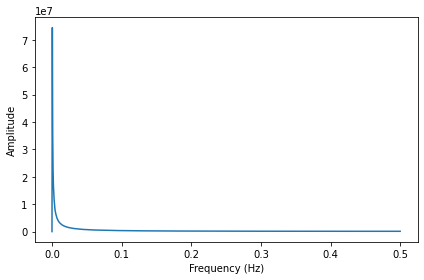
\includegraphics[width=0.7\linewidth]{resources/Images/task1_out_spectrum}
        \caption{Спектр выходного сигнала.}
        \label{fig:task1_out_spectrum}
    \end{figure}

    Получим отношение между входными и выходными данными.

    \begin{lstlisting}[caption= Получение отношения между входными и выходными данными., label={lst:task1_out_spectrum}]
sum(in_spectrum.amps < 1), len(in_spectrum)
ratio_spectrum = out_spectrum.ratio(in_spectrum, thresh=1)
ratio_spectrum.plot(marker='.', ms=4, ls='')
decorate(xlabel='Frequency (Hz)', ylabel='Amplitude ratio', yscale='log')  \end{lstlisting}

    \begin{figure}[H]
        \centering
        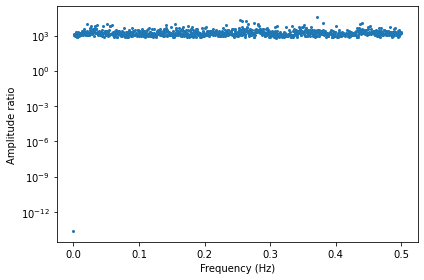
\includegraphics[width=0.7\linewidth]{resources/Images/task1_ratio_spectrum}
        \caption{Отношение между входными и выходными данными.}
        \label{fig:task1_out_spectrum}
    \end{figure}

    Теперь получим фильтр \texttt{cumsum} и интеграционный фильтр и сравним их.

    \begin{lstlisting}[caption= Вычисление фильтра \texttt{cumsum} и интеграционного фильтра., label={lst:task1_cumsum_integ_filters}]
diff_window = numpy.array([1.0, -1.0])
padded = zero_pad(diff_window, len(in_wave))
diff_wave = Wave(padded, framerate=in_wave.framerate)
diff_filter = diff_wave.make_spectrum()

cumsum_filter = diff_filter.copy()
cumsum_filter.hs[1:] = 1 / cumsum_filter.hs[1:]
cumsum_filter.hs[0] = numpy.inf

PI2 = numpy.pi * 2
integ_filter = cumsum_filter.copy()
integ_filter.hs[1:] = integ_filter.framerate / (PI2 * 1j * integ_filter.fs[1:])
integ_filter.hs[0] = numpy.inf

cumsum_filter.plot(label='cumsum filter', alpha=0.7)
integ_filter.plot(label='integral filter', alpha=0.7)
decorate(xlabel='Frequency (Hz)', ylabel='Amplitude ratio', yscale='log')  \end{lstlisting}

    \begin{figure}[h]
        \centering
        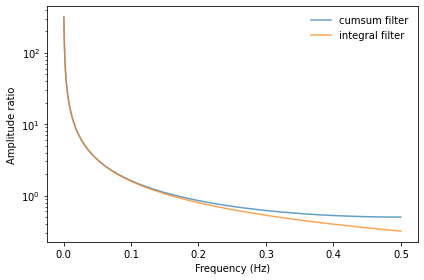
\includegraphics[width=0.8\linewidth]{resources/Images/task1_cumsum_integ_filters}
        \caption{Сравнение фильтров.}
        \label{fig:task1_cumsum_integ_filters}
    \end{figure}

    Теперь сравним вычисленные отношения с фильтром.

    \begin{lstlisting}[caption= Сравнение отношений с фильтром., label={lst:task1_cumsum_filter_ratio_spectrum}]
cumsum_filter.plot(label='cumsum filter')
ratio_spectrum.plot(label='ratio', marker='.', ms=4, ls='')
decorate(xlabel='Frequency (Hz)', ylabel='Amplitude ratio', yscale='log')  \end{lstlisting}

    \begin{figure}[H]
        \centering
        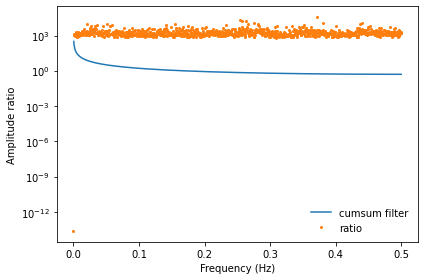
\includegraphics[width=0.65\linewidth]{resources/Images/task1_cumsum_filter_ratio_spectrum}
        \caption{Сравнение отношений с фильтром \texttt{cumsum}.}
        \label{fig:task1_cumsum_filter_ratio_spectrum}
    \end{figure}

    Тут уже можно заметить различия: графики не совпадают, хотя должны. Их совпадение подвердило бы, что фильтр
    \texttt{cumsum} является обратным фильтру \texttt{diff}.

    Теперь вычислим выходной сигнал, используя теорему свертки и сравним результаты.

    \begin{lstlisting}[caption= Вычисление выходного \texttt{wave}., label={lst:task1_compare_out_waves}]
len(in_spectrum), len(cumsum_filter)
out_wave.plot(label='summed', alpha=0.7)
cumsum_filter.hs[0] = 0
out_wave2 = (in_spectrum * cumsum_filter).make_wave()
out_wave2.plot(label='filtered', alpha=0.7)
decorate(xlabel='Time (s)') \end{lstlisting}

    \begin{figure}[H]
        \centering
        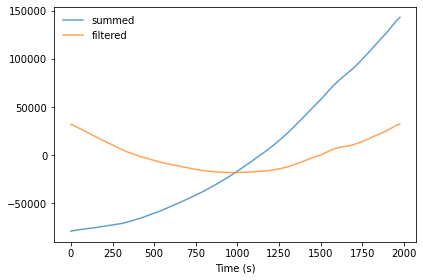
\includegraphics[width=0.65\linewidth]{resources/Images/task1_compare_out_waves}
        \caption{Сравнение выходных сигналов.}
        \label{fig:task1_compare_out_waves}
    \end{figure}

    Можно заметить, что выходные сигналы, полученные разными способами, не совпадают.
    Такое поведение говорит о некорректной работе примеров с апериодическими сигналами.

    В данном упражнении были изучены примеры в файле \texttt{chap09.ipynb}. После этого был проведён следующий эксперимент:
    периодический пилообразный сигнал был заменён на непериодические данные Facebook.
    В ходе эксперимента выяснилось, что некоторые примеры действительно работают некорректно с апериодическими сигналами.

    \newpage

% ---------------------------------------------- Упражнение 9.2 ----------------------------------------------
    \section{Упражнение 9.2}
    \label{sec:task2}

    В этом упражнении изучается влияние \texttt{diff} и \texttt{differentiate} на сигнал.

    Итак, начнём с создания треугольного сигнала.

    \begin{lstlisting}[caption= Создание треугольного сигнала., label={lst:task2_in_triangle}]
in_wave = TriangleSignal(freq=50).make_wave(duration=0.1, framerate=44100)
in_wave.plot()
decorate(xlabel='Time (s)')     \end{lstlisting}

    \begin{figure}[h]
        \centering
        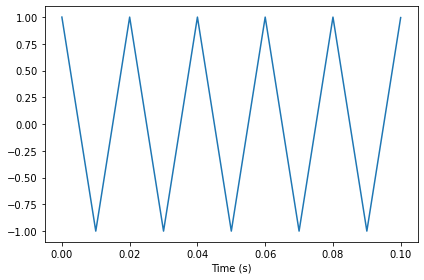
\includegraphics[width=0.8\linewidth]{resources/Images/task2_in_triangle}
        \caption{Треугольный сигнал.}
        \label{fig:task2_in_triangle}
    \end{figure}

    Теперь применим \texttt{diff} к нашему сигналу.

    \begin{lstlisting}[caption= Применение \texttt{diff}., label={lst:task2_out_dif}]
out_wave = in_wave.diff()
out_wave.plot()
decorate(xlabel='Time (s)') \end{lstlisting}

    \begin{figure}[h]
        \centering
        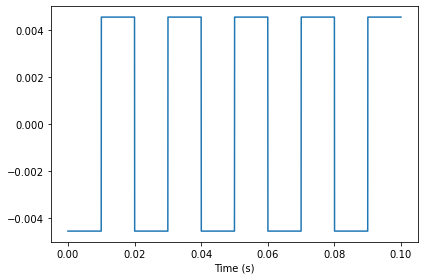
\includegraphics[width=0.7\linewidth]{resources/Images/task2_out_dif}
        \caption{Результат после применения \texttt{diff}.}
        \label{fig:task2_out_dif}
    \end{figure}

    Теперь посмотрим, как на сигнал повлияет \texttt{differentiate}. Для этого получим спектр треугольного сигнала и
    применим к нему \texttt{differentiate}. После чего преобразуем полученный результат обратно в \texttt{wave}.

    \begin{lstlisting}[caption= Применение \texttt{differentiate}., label={lst:task2_out_differentiate}]
out_wave2 = in_wave.make_spectrum().differentiate().make_wave()
out_wave2.plot()
decorate(xlabel='Time (s)')     \end{lstlisting}

    \begin{figure}[H]
        \centering
        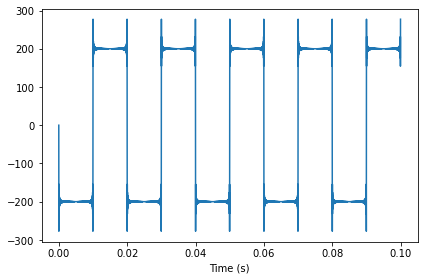
\includegraphics[width=0.7\linewidth]{resources/Images/task2_out_differentiate}
        \caption{Результат после применения \texttt{differentiate}.}
        \label{fig:task2_out_differentiate}
    \end{figure}

    Когда мы берем спектральную производную, мы получаем "звон" вокруг разрывов.
    С математической точки зрения проблема в том, что производная треугольной волны не определена в точках треугольника.

    В данном упражнении было изучено влияние \texttt{diff} и \texttt{differentiate} на сигнал.
    Был сделан вывод, что при взятии спектральной производной треугольного сигнала получается "звон" вокруг разрывов.
    Это проблема возникает из-за того, что производная треугольной волны не определена в точках треугольника.

    \newpage

% ---------------------------------------------- Упражнение 9.3 ----------------------------------------------
    \section{Упражнение 9.3}
    \label{sec:task3}

    В этом упражнении изучается влияние \texttt{cumsum} и \texttt{integrate} на сигнал.

    Для начала создадим прямоугольный сигнал.

    \begin{lstlisting}[caption= Создание прямоугольного сигнала., label={lst:task3_in_square}]
in_wave = SquareSignal(freq=50).make_wave(duration=0.1, framerate=44100)
in_wave.plot()
decorate(xlabel='Time (s)')     \end{lstlisting}

    \begin{figure}[h]
        \centering
        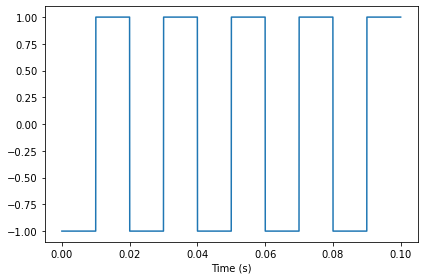
\includegraphics[width=0.8\linewidth]{resources/Images/task3_in_square}
        \caption{Прямоугольный сигнал.}
        \label{fig:task3_in_square}
    \end{figure}

    Теперь применим к нашему сигналу \texttt{cumsum} и посмотрим на результат.

    \begin{lstlisting}[caption= Применение \texttt{cumsum}., label={lst:task3_out_cumsum}]
out_wave = in_wave.cumsum()
out_wave.plot()
decorate(xlabel='Time (s)')     \end{lstlisting}

    Как мы видим из Рис.\ref{fig:task3_out_cumsum}, совокупная сумма прямоугольного сигнала - это треугольный сигнал.

    \begin{figure}[H]
        \centering
        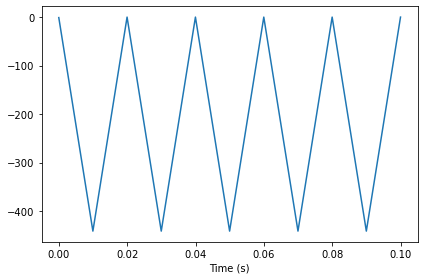
\includegraphics[width=0.7\linewidth]{resources/Images/task3_out_cumsum}
        \caption{Результат после применения \texttt{cumsum}.}
        \label{fig:task3_out_cumsum}
    \end{figure}

    Теперь вычислим спектр нашего прямоугольного сигнала и применим к нему \texttt{integrate}.

    \begin{lstlisting}[caption= Применение \texttt{integrate}., label={lst:task3_out_integrate}]
spectrum = in_wave.make_spectrum().integrate()
spectrum.hs[0] = 0
out_wave2 = spectrum.make_wave()
out_wave2.plot()
decorate(xlabel='Time (s)')     \end{lstlisting}

    \begin{figure}[h]
        \centering
        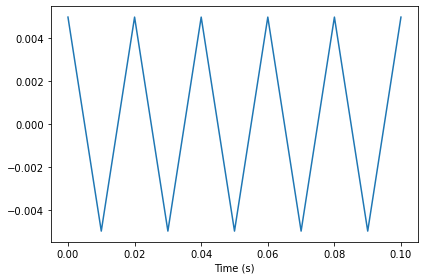
\includegraphics[width=0.7\linewidth]{resources/Images/task3_out_integrate}
        \caption{Результат после применения \texttt{integrate}.}
        \label{fig:task3_out_integrate}
    \end{figure}

    Из Рис.\ref{fig:task3_out_integrate} видно, что спектральный интеграл также является треугольным сигналом.
    У полученных сигналов, однако, сильно отличается амплитуда.

    Попробуем уравновесить и нормализовать оба сигнала.

    \begin{lstlisting}[caption= Работа с сигналами., label={lst:task3_normalize_result}]
out_wave.unbias()
out_wave.normalize()
out_wave2.normalize()
out_wave.plot()
out_wave2.plot()
out_wave.max_diff(out_wave2)    \end{lstlisting}

    \begin{figure}[h]
        \centering
        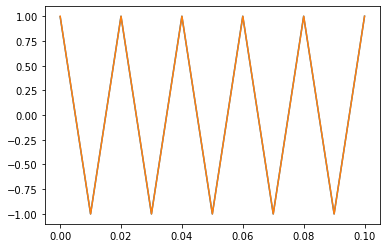
\includegraphics[width=0.8\linewidth]{resources/Images/task3_normalize_result}
        \caption{Сравнение полученных сигналов.}
        \label{fig:task3_normalize_result}
    \end{figure}

    Теперь они визуально похожи. Их же максимальная разница (\texttt{0.0045351473922902175}) говорит о том, что их
    численное значение похоже с точностью до 2 знаков после запятой.

    В данном упражнении было изучено влияние \texttt{cumsum} и \texttt{integrate} на сигнал. Для этого был создан
    прямоугольный сигнал, к которому по очереди были применены эти функции. По полученным результатам был сделан вывод,
    что совокупная сумма и спектральный интеграл прямоугольного сигнала очень похожи. При их нормализации можно увидеть,
    что их значения похожи с точностью до 2 знаков после запятой.

    \newpage

% ---------------------------------------------- Упражнение 9.4 ----------------------------------------------
    \section{Упражнение 9.4}
    \label{sec:task4}

    В данном упражнении изучается влияние двойного интегрирования.

    Начнём с создания пилообразного сигнала.

    \begin{lstlisting}[caption= Создание пилообразного сигнала., label={lst:task4_in_sawtooth}]
in_wave = SawtoothSignal(freq=50).make_wave(duration=0.1, framerate=44100)
in_wave.plot()
decorate(xlabel='Time (s)')     \end{lstlisting}

    \begin{figure}[h]
        \centering
        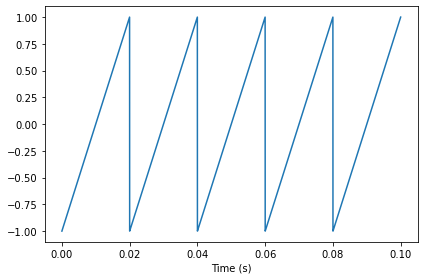
\includegraphics[width=0.8\linewidth]{resources/Images/task4_in_sawtooth}
        \caption{Пилообразный сигнал.}
        \label{fig:task4_in_sawtooth}
    \end{figure}

    Теперь применим \texttt{integrate} к нашему сигналу.

    \begin{lstlisting}[caption= Применение \texttt{integrate}., label={lst:task4_out_integrate_1}]
spectrum = in_wave.make_spectrum().integrate()
spectrum.hs[0] = 0
out_wave = spectrum.make_wave()
out_wave.plot()
decorate(xlabel='Time (s)')     \end{lstlisting}

    Как мы видим из Рис.\ref{fig:task4_out_integrate_1}, первый спектральный интеграл - это парабола.

    Повторно применим \texttt{integrate} и посмотрим на результат.

    \begin{lstlisting}[caption= Второе применение \texttt{integrate}., label={lst:task4_out_integrate_2}]
spectrum2 = spectrum.integrate()
spectrum2.hs[0] = 0
out_wave2 = spectrum2.make_wave()
out_wave2.plot()
decorate(xlabel='Time (s)')     \end{lstlisting}

    \begin{figure}[H]
        \centering
        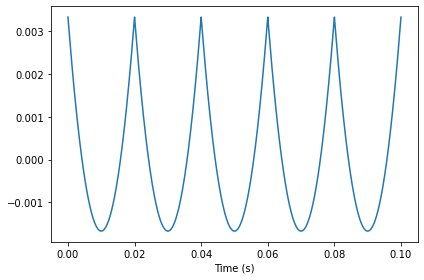
\includegraphics[width=0.8\linewidth]{resources/Images/task4_out_integrate_1}
        \caption{Сигнал после первого применения \texttt{integrate}.}
        \label{fig:task4_out_integrate_1}
    \end{figure}

    \begin{figure}[H]
        \centering
        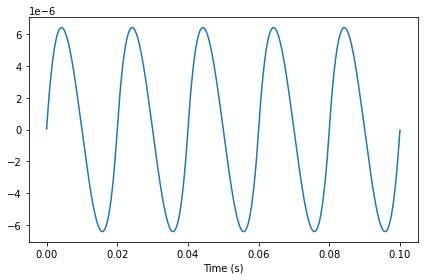
\includegraphics[width=0.8\linewidth]{resources/Images/task4_out_integrate_2}
        \caption{Сигнал после второго применения \texttt{integrate}.}
        \label{fig:task4_out_integrate_2}
    \end{figure}

    Как мы видим, двойное интегрирование даёт кубическую кривую.

    Результат напоминает синусоиду. Это связано с тем, что интегрирование действует как фильтр нижних частот.
    Посмотрим, какие частоты у нас остались.

    \begin{lstlisting}[caption= Получение спектра., label={lst:task4_spectrum_after}]
out_wave2.make_spectrum().plot(high=500)    \end{lstlisting}

    \begin{figure}[h]
        \centering
        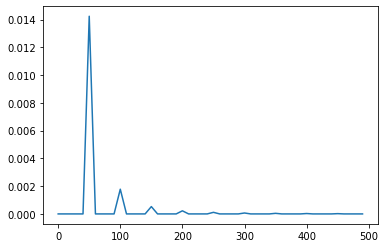
\includegraphics[width=0.8\linewidth]{resources/Images/task4_spectrum_after}
        \caption{Спектр полученного сигнала.}
        \label{fig:task4_spectrum_after}
    \end{figure}

    Из рисунка выше (Рис.\ref{fig:task4_spectrum_after}) видно, что мы отфильтровали почти всё, кроме основного.

    В данном упражнении было изучено влияние двойного интегрирования на сигнал. Для этого был создан
    пилообразный сигнал, к которому два раза был применён \texttt{integrate}. По полученным результатам был сделан вывод,
    что интегрирование действует как фильтр нижних частот.

    \newpage

% ---------------------------------------------- Упражнение 9.5 ----------------------------------------------
    \section{Упражнение 9.5}
    \label{sec:task5}

    В этом упражнении изучается влияние второй разности и второй производной.

    Начнём с создания кубического сигнала.

    \begin{lstlisting}[caption= Кубический сигнал., label={lst:task5_in_cubic}]
in_wave = CubicSignal(freq=0.0005).make_wave(duration=10000, framerate=1)
in_wave.plot()      \end{lstlisting}

    \begin{figure}[h]
        \centering
        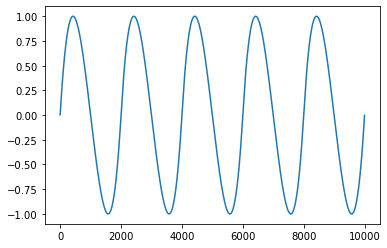
\includegraphics[width=0.8\linewidth]{resources/Images/task5_in_cubic}
        \caption{Кубический сигнал.}
        \label{fig:task5_in_cubic}
    \end{figure}

    Теперь вычислим вторую разность, дважды применив \texttt{diff}.

    \begin{lstlisting}[caption= Двойное примнение \texttt{diff}., label={lst:task5_out_diff}]
out_wave = in_wave.diff().diff()
out_wave.plot()     \end{lstlisting}

    Результат второго применения - пилообразная волна.

    Теперь вычислим вторую производную, дважды применив \texttt{differentiate}

    \begin{lstlisting}[caption= Двойное примнение \texttt{differentiate}., label={lst:task5_out_differentiate}]
out_wave = in_wave.diff().diff()
out_wave.plot()     \end{lstlisting}

    \begin{figure}[H]
        \centering
        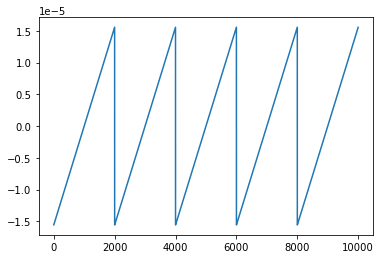
\includegraphics[width=0.8\linewidth]{resources/Images/task5_out_diff}
        \caption{Сигнал после двойного применения \texttt{diff}.}
        \label{fig:task5_out_diff}
    \end{figure}

    \begin{figure}[H]
        \centering
        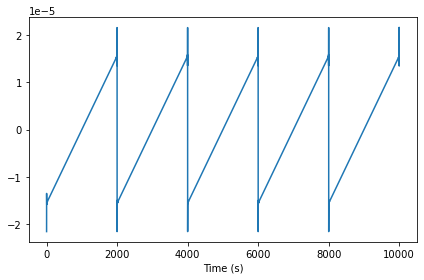
\includegraphics[width=0.8\linewidth]{resources/Images/task5_out_differentiate}
        \caption{Сигнал после двойного применения \texttt{differentiate}.}
        \label{fig:task5_out_differentiate}
    \end{figure}

    Видно, что в результате двойного дифференцирования был получен пилообразный сигнал со "звоном".
    Как мы уже выяснили, это связано с тем, что производная параболического сигнала не определена в точках.

    Теперь рассчитаем фильтры, соответствующие второй разнице и второй производной, и сравним их.

    \begin{lstlisting}[caption= Вычисление фильтра для второй разности., label={lst:task5_diff_filter}]
diff_window = numpy.array([-1.0, 2.0, -1.0])
padded = zero_pad(diff_window, len(in_wave))
diff_wave = Wave(padded, framerate=in_wave.framerate)
diff_filter = diff_wave.make_spectrum()     \end{lstlisting}

    \begin{lstlisting}[caption= Вычисление фильтра для второй производной и сравнение фильтров., label={lst:task5_deriv_filter}]
deriv_filter = in_wave.make_spectrum()
deriv_filter.hs = (PI2 * 1j * deriv_filter.fs)**2

diff_filter.plot(label='2nd diff')
deriv_filter.plot(label='2nd deriv')
decorate(xlabel='Frequency (Hz)', ylabel='Amplitude ratio')     \end{lstlisting}

    \begin{figure}[h]
        \centering
        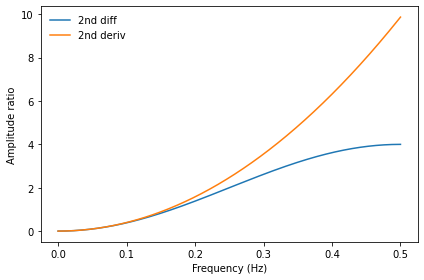
\includegraphics[width=0.8\linewidth]{resources/Images/task5_compare_filters}
        \caption{Сравнение фильтров.}
        \label{fig:task5_compare_filters}
    \end{figure}

    Как мы видим из Рис.\ref{fig:task5_compare_filters}, оба фильтра - фильтры высоких частот, усиливающие компоненты
    самых высоких частот. Вторая производная - параболическая, поэтому она сильнее всего усиливает самые высокие частоты.
    Вторая разница очень близка к второй производной на низких частотах, однако потом достаточно сильно отклоняется от
    неё.

    В данном упражнении было изучено влияние второй разности и второй производной на сигнал. Для этого был создан
    кубический сигнал, для которого были получены вторая разность и вторая производная. Их результат - пилообразный
    сигнал. Однако для второй производной сигнал получился со "звоном". Затем для них были вычислены фильтры.
    При сравнении полученных фильтров был сделан вывод, что вторая производная усиливает высокие частоты сильнее, чем
    вторая разница.

    \newpage

% ---------------------------------------------- Выводы ----------------------------------------------
    \section{Выводы}
    \label{sec:conclusions}

    В ходе выполнения данной лабораторной работы были изучены дифференцирование и интегрирование и их влияние на сигнал.
    Был сделан вывод, что интегрирование действует как фильтр нижних частот, а дифференцирование усиливает
    высокие частоты. Также был сделан вывод, что результат совокупной суммы и спектрального интеграла очень похожи.

    Кроме того, важно помнить, что при взятии производных сигнал часто получается со "звоном".

\end{document}